% visual
\بخش{بینایی ماشین در \جام}
در تحقیق که در \سال{2010} بروی ترکیب اطلاعات سنسور لیزری دامنه‌یاب\زیرنویس{\مق{Laser Range Finder}} و اطلاعات حاصل از دوربین استریو صورت گرفت\مرجع{kumar2010sensor} در این تحقیق که بر روی یک ربات زمینی پیاده‌سازی شد برای افزایش سرعت محاسباتی از اطلاعات عمقی بدست آمده دوربین‌ها قسمتی از اطلاعات را که بیشتر از یک ارتفاع مشخص از زمین را دارد دور می‌ریزد سپس یک نقشه‌ی ۲بعدی از نواحی اشغالی از تصاویر ۳بعدی و در نهایت با ترکیب اطلاعات سنسور لیزری و نقشه‌ی دوبعدی بدست آمده از دوربین‌های استریو، نقشه‌ی ۲بعدی اشفالی از محیط را می‌سازد و به الگوریتم \مق{VFH+} بجهت راهبری و \جام می‌دهد.\بند

در \سال{2013} در پژوهشی\مرجع{peasley2013real} با استفاده از سنسور سه‌بعدی کینکت\زیرنویس{Kinect} در چهار مرحله اقدام به تشخیص مانع می‌کند، در مرحله‌ی نخست اطلاعات عمقی از سنسور کینکت به یک فضای ۳بعدی با استفاده از اطلاعات کالیبراسیون\زیرنویس{Calibration} سنسور منتقل می‌شود. در مرحله‌ی دوم صفحه‌ی زمین در این فضا تشخیص و حذف می‌شود، در مرحله‌ی سوم یک نقشه‌ی ۲بعدی فضای اشغالی\زیرنویس{\مق{Occupancy Map}} با تصویر کردن\زیرنویس{Projecting} این نقشه به نمای بالابه‌پایین\زیرنویس{Top-Down View} ساخته می‌شود و در مرحله‌ی آخر الگوریتم \جام با استفاده از این نقشه‌ی فضای اشغالی تصمیم میگیرد که چگونه ربات را کنترل کند. در این پژوهش تمرکز اصلی بروی تشخیص مانع گذاشته شده است زیرا که برای الگوریتم \جام به صورت یک حالت کلی بحث شده است.\بند

\begin{figure}[b]
\centering
\subfigure[تصویر دوربین سمت چپ]{ 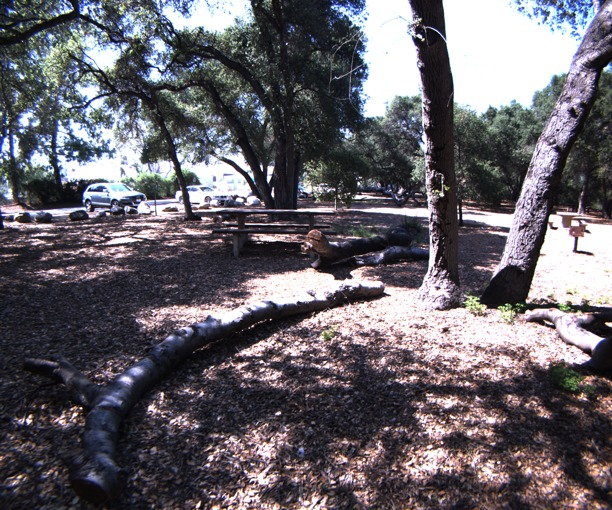
\includegraphics[width=.3\textwidth]{cexp-1}\label{fig:cexp_1} }
\subfigure[نقشه‌ی اختلاف -- هرچه رنگ تیره‌تر(متمایل به قرمز و آبی) اختلاف و جابجایی پیکسل‌ها در تصویر دوربین سمت چپ و راست کمتر و عمق بیشتر.]{ 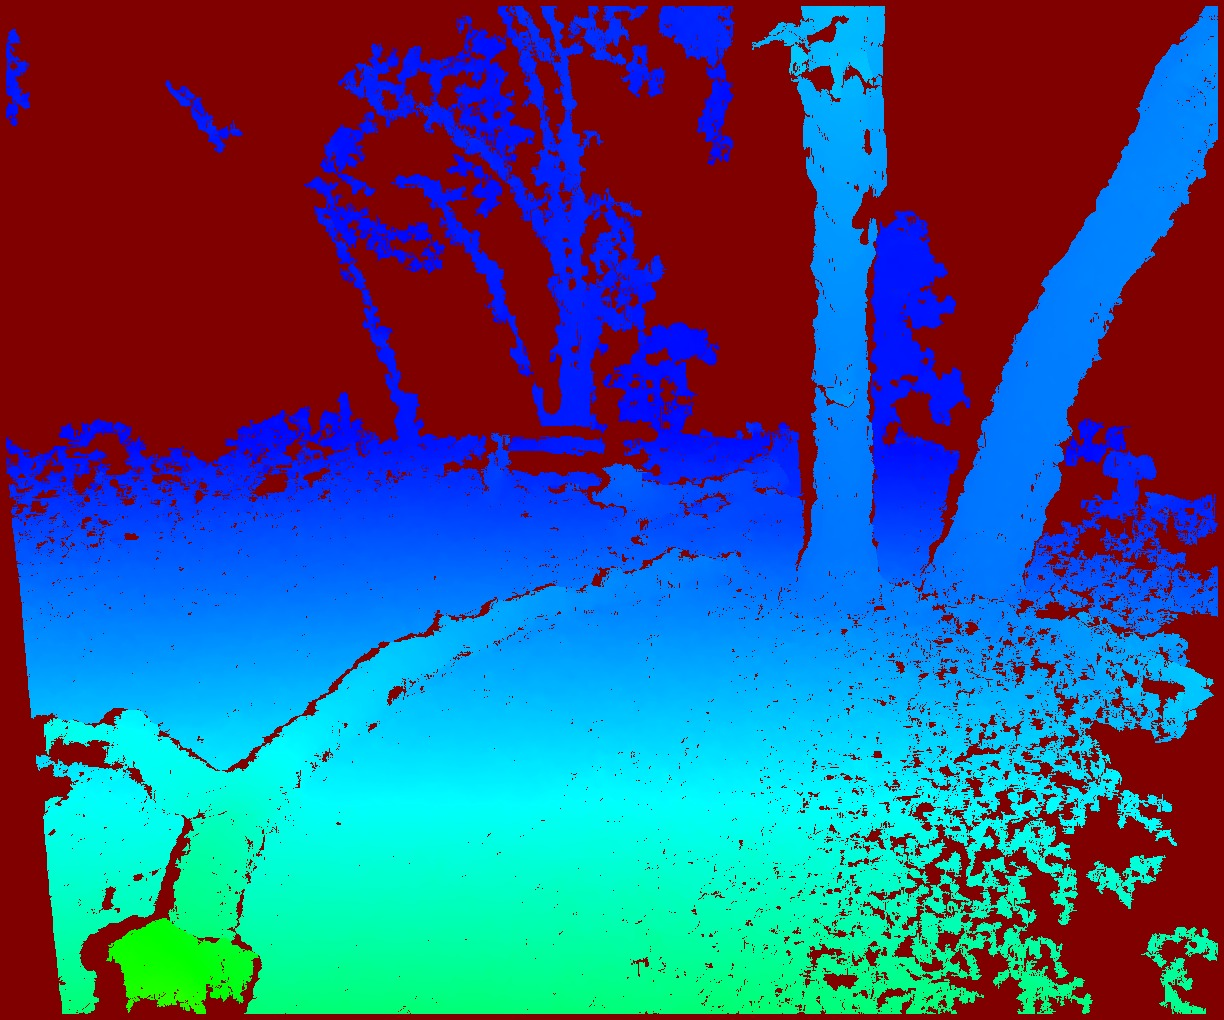
\includegraphics[width=.3\textwidth]{cexp-2}\label{fig:cexp_2} }
\subfigure[نقشه‌ی جابجایی گسترش داده شده]{ 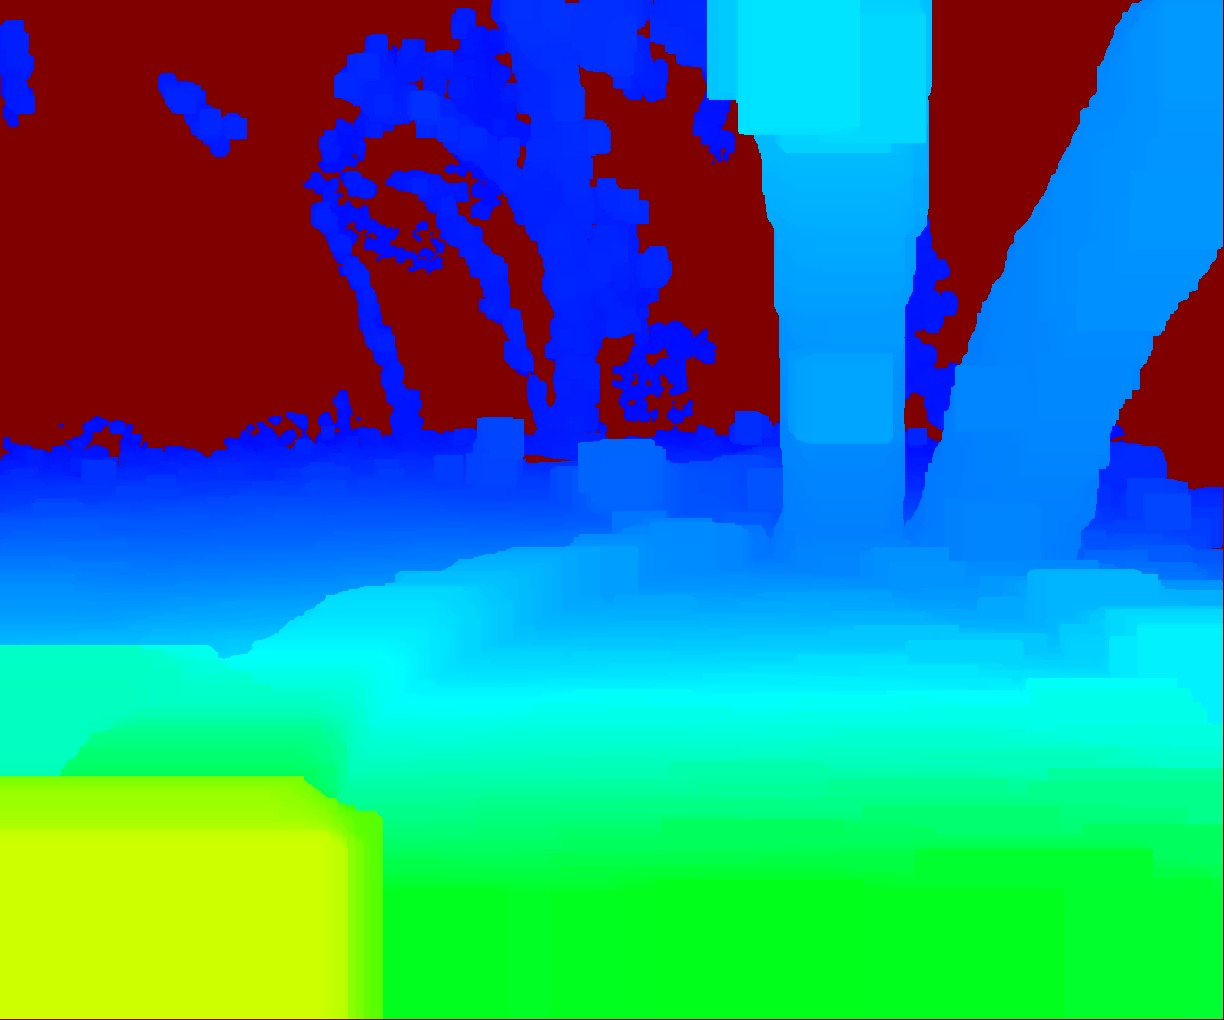
\includegraphics[width=.3\textwidth]{cexp-3}\label{fig:cexp_3} }
\caption{گسترش
\مق{C-Space}
در فضای نقشه‌ی اختلاف}
\label{fig:c_space_expansion}
\end{figure}

پژوهشی دیگر بروی \جام بر مبنای تصویر بروی یک ربات چهارپره در \سال{2014} انجام شد\مرجع{matthies2014stereo}. در این تحقیق \جام به‌سبب بهینگی در پردازش داده و امکان پردازش و راهبری برخط ربات در سطح نقشه‌ی اختلاف\زیرنویس{\مق{Disparity Map}}(که از مراحل اولیه عمق سنجی با استفاده از تصاویر استریو می‌باشد) صورت گرفته است. این پژوهش گسترشی\زیرنویس{Expansion} به‌نام \مق{C-Space Expansion} معرفی کرده است که بصورت متناسب ابعاد جابجایی نواحی موجود در نقشه‌ی اختلاف را گسترده می‌کند که در نهایت کمک میکند تا اغتشاش‌های موجود در نقشه حذف گردد و نقشه را بتوان به چند قطعه\زیرنویس{Segment} عمده شکست و حفره‌های فرار از موانع را تشخیص داد(شکل \ref{fig:c_space_expansion}). در این مقاله بجهت راهبری از تکنیک نقاط‌مسیر که در قسمت‌های قبلی آورده شده است، استفاده می‌کند.\بند

پژوهشی\مرجع{barry2015pushbroom} در \سال{2015} به ارائه‌ی الگوریتمی سریع برای شناسایی و \جام در پهپادهایی با سرعت پرواز بالا ارائه داد. ایده‌ای که این مقاله داده جالب است و مساله‌ی استخراج نقشه‌ی اختلاف و تطبیق بلوک\زیرنویس{\مق{Block Matching}} را به جستجو میان اعماق تعریف کرده است. حال با محدود کردن جستجوی میزان جابجایی بلوک‌ها، می‌توان فقط به شناسایی اشیایی که در یک فاصله‌ی معین قراردارند پرداخت و به ازای در نظر نگرفتن اشیایی که در فاصله‌ای غیر از این قرار دارند،میتوان سرعت الگوریتم را بصورت توانی افزایش داد. در نهایت با استفاده از ادومتری پهپاد و اطلاعات تجمعی حاصل از این تطبیق الگوهای محدود می‌توان اطلاعات فاصله‌ی پیکسل‌هایی که از قبل از و فاصله‌ی دور شناسایی شده‌اند را بازسازی کند(شکل \ref{fig:pushbroom}).\بند

\fig[.17]{pushbroom}{تشخیص عمق در یک عمق مشخص(رنگ آبی‌تیره) و ادغام ادومتری پهپاد و تشخیص‌های قبلی(رنگ‌های آبی روشن‌تر) به سرعت می‌توان نقشه‌ی کاملی از موانع مقابل پهپاد ساخت.}

در تحقیقی که در \سال{2016} بروی راهبری مبتنی بر تصاویر استریو\مرجع{van2016persistent} صورت گرفت که تلاشی در راستای یادگیری خود-مختاری ربات‌های پرنده با رویکرد راهبری تصویری\زیرنویس{\مق{Visual Navigation}} به جهت \جام می‌باشد. در این تحقیق با استفاده از دو دوربین استریو تصاویر، نقشه‌ی اختلاف قالب\زیرنویس{Frame}‌های این دو دوربین را بدست می‌آورند، سپس با استفاده از یک تخمین‌زن نقشه‌ی عدم شباهت بروی تصویر سمت چپ مدلی را یادگرفته و بعد از گذرانده شدن از فیلتری به واحد تصمیم‌گیری ارسال می‌گردد. در حین یادگیری تخمین‌‌زن نقشه مشغول به یادگیری می‌باشد ولی بعد از دوره‌ی یادگیری فقط با استفاده از تصاویر دوربین سمت چپ و تخمین‌زن به تصمیم‌گیری می‌پردازد و فقط در صورتی که تخمین‌زن در انجام وظیفه‌ی خود شکست بخورد و نتواند تخمینی معتبر ارائه دهد با استفاده از تصاویر استریو از تصادف جلوگیری به عمل می‌آید؛ با این روش از سربار محاسباتی‌ای که هربار توسط پردازش تصاویر استریو به عمل می‌آید جلوگیری می‌شود.\بند